\documentclass[../main.tex]{subfiles}

\begin{document}

\justifying

\section{Analizar úncamente el potencial de tres cuerpos}

Está la cofniguración tres en prueba.

\subsection{Directory: 2026-03-04-095332}

La tabla tiene la siguiente configuración:
\begin{align*}
    F_{1} &= f_{1}\hat{r}_{12} + f_{2}\hat{r}_{13} \\
    f_{i1} &= f_{1} \\
    f_{i2} &= f_{2} \\
    f_{j2} &= 0
\end{align*}
Si lo de lammps y la teórica son lo mismo, esto indica que la tabla es la fuerza por partícula y lammps le asigana individualmente a cada partícula en el triplete la fuerza.


\begin{figure}[!ht]
    \centering
    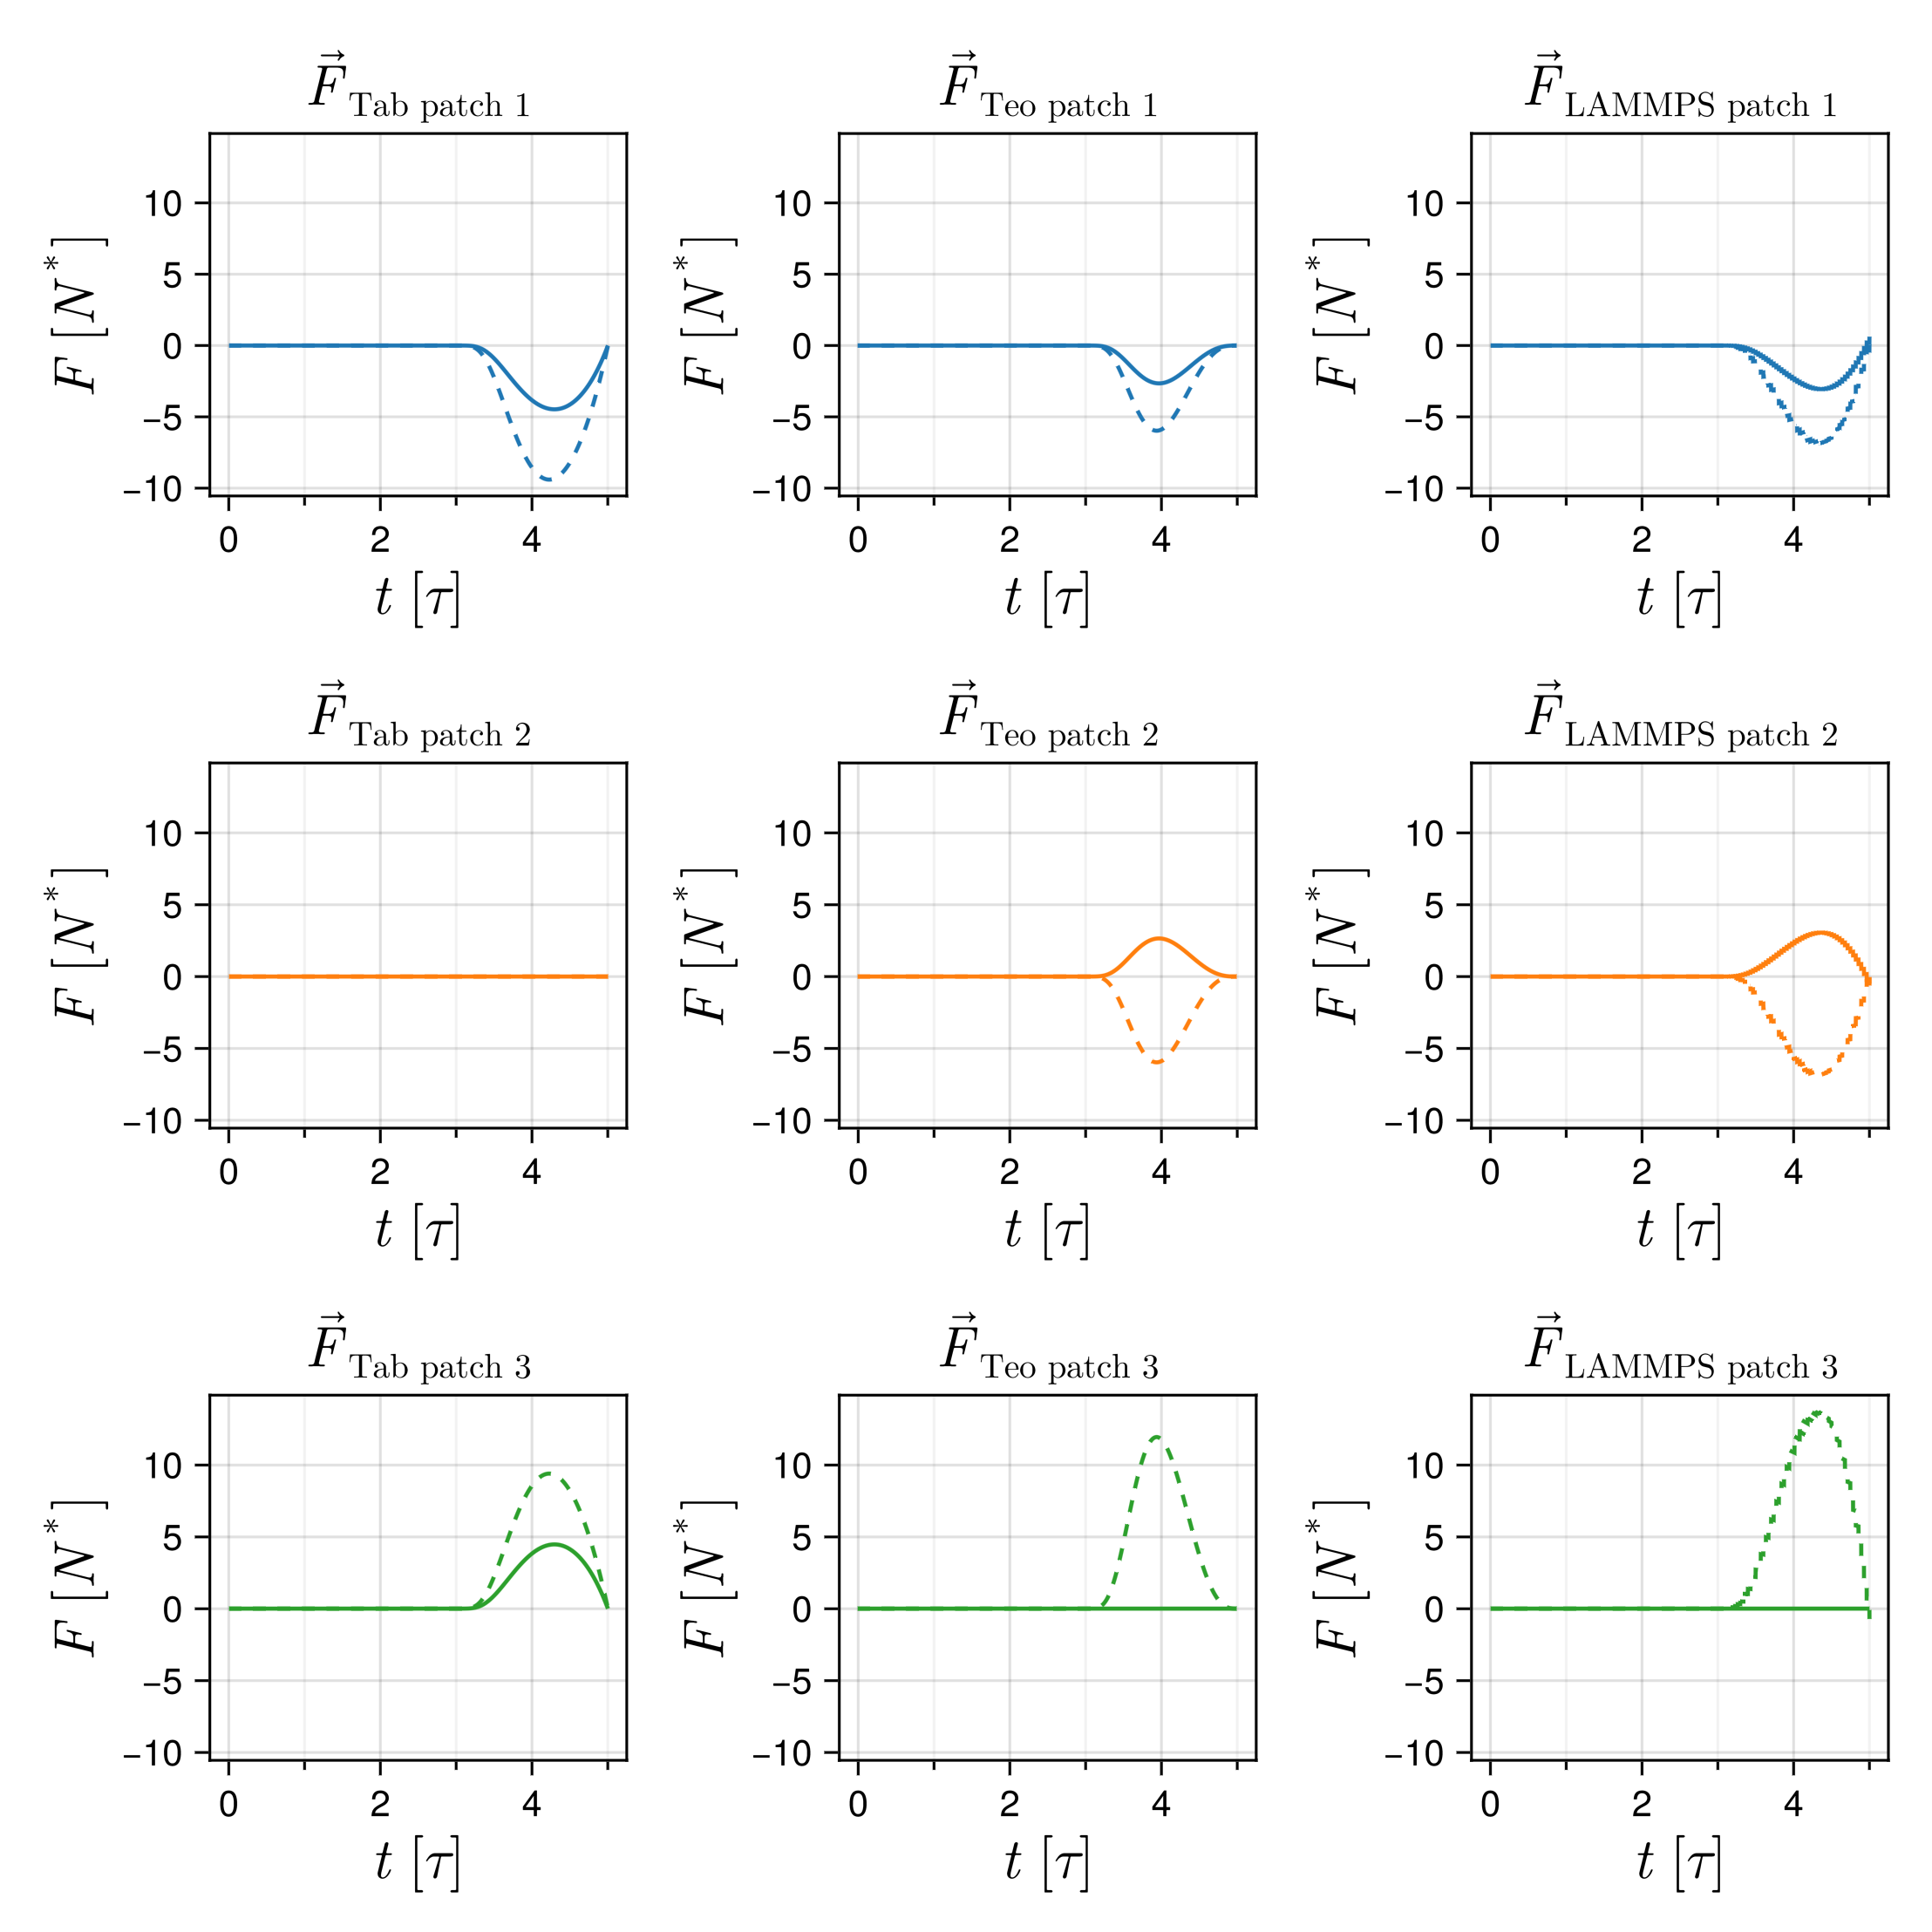
\includegraphics[width=\textwidth]{../Figures/2026-03-04-095332/fig_FTabTeo.png}
    \caption{
        Línea sólida: Componente $x$, línea punteada: Componente $y$.
        Línea azul: particula central.
        Línea naranja: partícula superior.
        Línea verde: partícula inferior.
    }\label{fig:Config3-TabTeo}
\end{figure}

\newpage

La columan de la izquierda muestra las fuerzas calculadas de la siguiente forma:
\begin{gather}
    \begin{pmatrix}
        \vec{f}_1 \\ \vec{f}_2 \\\vec{f}_3 
    \end{pmatrix}
    =
    \begin{pmatrix}
        f_{i1} & f_{i2} & 0 \\
        -f_{i1} & 0 & 0 \\
        0 & -f_{i2} & 0
    \end{pmatrix}
    \begin{pmatrix}
        \vec{r}_{12} \\ \vec{r}_{13} \\\vec{r}_{23} 
    \end{pmatrix}
    \label{eqn:lammps3body}
\end{gather}

La columna central se muetra el análisis teórico del potencial de 3 cuerpos,
\marginnote{
%\begin{align*}
%    \vec{F}_{\mathrm{swap}-1} &= w\epsilon_{2,3}\left[
%        U_3(r_{1,3})f_3(r_{1,2})\hat{r}_{1,2} + U_3(r_{1,2})f_3(r_{1,3})\hat{r}_{1,3}
%    \right] \\
%    \vec{F}_{\mathrm{swap}-2} &= w\epsilon_{1,3}\left[
%        -U_3(r_{2,3})f_3(r_{2,1})\hat{r}_{1,2} + U_3(r_{2,1})f_3(r_{2,3})\hat{r}_{2,3}
%    \right] \\
%    \vec{F}_{\mathrm{swap}-3} &= w\epsilon_{1,2}\left[
%            -U_3(r_{3,2})f_3(r_{3,1})\hat{r}_{1,3} - U_3(r_{3,1})f_3(r_{3,2})\hat{r}_{2,3}
%    \right]
%\end{align*}

    \begin{align*}
    f_{12s} &= w\epsilon_{2,3}U_3(r_{1,3})f_3(r_{1,2}) \\
    f_{13s} &= w\epsilon_{2,3}U_3(r_{1,2})f_3(r_{1,3}) \\
    f_{21s} &= w\epsilon_{1,3}U_3(r_{2,3})f_3(r_{2,1}) \\
    f_{23s} &= w\epsilon_{1,3}U_3(r_{2,1})f_3(r_{2,3}) \\
    f_{31s} &= w\epsilon_{1,2}U_3(r_{3,2})f_3(r_{3,1}) \\
    f_{32s} &= w\epsilon_{1,2}U_3(r_{3,1})f_3(r_{3,2})
\end{align*}
}
\begin{align*}
    \vec{F}_1 &= \qty(f_{12s} - f_{21s})\hat{r}_{12} + \qty(f_{13s} - f_{31s})\hat{r}_{13} \\
    \vec{F}_2 &= \qty(f_{21s} - f_{12s})\hat{r}_{21} + \qty(f_{23s} - f_{32s})\hat{r}_{23} \\
    \vec{F}_3 &= \qty(f_{31s} - f_{13s})\hat{r}_{31} + \qty(f_{32s} - f_{23s})\hat{r}_{32}
\end{align*}

Y en la última columna, aparece el resultado obtenido por LAMMPS.
Parece que LAMMPS asigna la fuerza a cada una de la partículas y después hace la sumatoria.

Por otro lado, comparando cualitativamente la clumna dos con la columna tres, para que los dominios están "volteados".
Cómo que si estuvieran en un espejo.

\newpage 

La partícula $i$ es la partícula 2.

\subsection{Directory: 2026-03-04-104032}
\begin{figure}[!ht]
    \centering
    
\includegraphics[width=\textwidth]{../Figures/2026-03-04-104032/fig_FTabTeo.png}
    \caption{
        Línea sólida: Componente $x$, línea punteada: Componente $y$.
        Línea azul: particula central.
        Línea naranja: partícula superior.
        Línea verde: partícula inferior.
    }\label{fig:Config3-TabTeo-2}
\end{figure}


\newpage 

La partícula $i$ es la partícula 3

\subsection{Directory: 2026-03-04-104950}
\begin{figure}[!ht]
    \centering
    
\includegraphics[width=\textwidth]{../Figures/2026-03-04-104950/fig_FTabTeo.png}
    \caption{
        Línea sólida: Componente $x$, línea punteada: Componente $y$.
        Línea azul: particula central.
        Línea naranja: partícula superior.
        Línea verde: partícula inferior.
    }\label{fig:Config3-TabTeo-3}
\end{figure}

\newpage 

Ahora la tabla es la suma de las fuerzas,
\begin{align*}
    \vec{F}_1 &= \qty(f_{12s} - f_{21s})\hat{r}_{12} + \qty(f_{13s} - f_{31s})\hat{r}_{13} \\
    \vec{F}_2 &= \qty(f_{21s} - f_{12s})\hat{r}_{21} + \qty(f_{23s} - f_{32s})\hat{r}_{23} \\
    \vec{F}_3 &= \qty(f_{31s} - f_{13s})\hat{r}_{31} + \qty(f_{32s} - f_{23s})\hat{r}_{32}
\end{align*}

\subsection{Directory: 2026-03-04-105941}
\begin{figure}[!ht]
    \centering
    
\includegraphics[width=\textwidth]{../Figures/2026-03-04-105941/fig_FTabTeo.png}
    \caption{
        Línea sólida: Componente $x$, línea punteada: Componente $y$.
        Línea azul: particula central.
        Línea naranja: partícula superior.
        Línea verde: partícula inferior.
    }\label{fig:Config3-TabTeo-4}
\end{figure}

Y pues ya dio la forma cualitativa.
Las magnitudes no cuadran.

\newpage

Se realiza lo siguiente \(\vec{F}_{\mathrm{Teo}} - \vec{F}_{\mathrm{LAMMPS}} / \vec{F}_{\mathrm{Teo}}\) para saber el factor de escalamiento.
\begin{figure}[!ht]
    \centering
    
\includegraphics[width=\textwidth]{../Figures/2026-03-04-105941/fig_FswapDiff.png}
    \caption{
        Línea sólida: Componente $x$, línea punteada: Componente $y$.
        Línea azul: particula central.
        Línea naranja: partícula superior.
        Línea verde: partícula inferior.
    }\label{fig:Config3-DiffTeoLAMMPS}
\end{figure}
Enfocando únicamente en el intervalo \(t\in[3.5,4.5]\), se obtiene un promedio de \(\approx 0.5\), indicando que hay un factor de 2.
Esto ocurre en ambas componentes.
No me queda muy claro de donde proviene este factor de dos, pero bueno.

\newpage 

\subsection{Direcotry: 2026-03-04-134835}
Le introdujé el valor de \(2\) a la tabla y ya todo salió decente.

\begin{figure}[!ht]
    \centering
    
\includegraphics[width=\textwidth]{../Figures/2026-03-04-134835/fig_FTabTeo.png}
    \caption{
        Línea sólida: Componente $x$, línea punteada: Componente $y$.
        Línea azul: particula central.
        Línea naranja: partícula superior.
        Línea verde: partícula inferior.
    }\label{fig:Config3-TabTeo-5}
\end{figure}

\newpage

Aquí está una comparación visual/cualitativa de las fuerzas.

\begin{figure}[!ht]
    \centering
    
\includegraphics[width=0.8\textwidth]{../Figures/2026-03-04-134835/fig_ForceComp.png}
    \caption{
        Línea sólida: Componente $x$, línea punteada: Componente $y$.
        Línea azul: particula central.
        Línea naranja: partícula superior.
        Línea verde: partícula inferior.
    }\label{fig:Config3-TabTeo-5}
\end{figure}

Acá va la diferencia entre la teorica y lo de LAMMPS,
\begin{figure}[!ht]
    \centering
    
\includegraphics[width=\textwidth]{../Figures/2026-03-04-134835/fig_FswapDiff.png}
    \caption{
        Línea sólida: Componente $x$, línea punteada: Componente $y$.
        Línea azul: particula central.
        Línea naranja: partícula superior.
        Línea verde: partícula inferior.
    }\label{fig:Config3-TabTeo-5}
\end{figure}

Voy a ver que ocurre si aumento de $2^7$ a $2^8$ puntos en la tabulación del potencial de 3 cuerpos.

\newpage

\subsection{Directory: 2026-03-04-141237}

\begin{figure}[!ht]
    \centering
    
\includegraphics[width=0.8\textwidth]{../Figures/2026-03-04-141237/fig_ForceComp.png}
    \caption{
        Línea sólida: Componente $x$, línea punteada: Componente $y$.
        Línea azul: particula central.
        Línea naranja: partícula superior.
        Línea verde: partícula inferior.
    }\label{fig:Config3-TabTeo-5}
\end{figure}

Acá va la diferencia entre la teorica y lo de LAMMPS,
\begin{figure}[!ht]
    \centering
    
\includegraphics[width=\textwidth]{../Figures/2026-03-04-141237/fig_FswapDiff.png}
    \caption{
        Línea sólida: Componente $x$, línea punteada: Componente $y$.
        Línea azul: particula central.
        Línea naranja: partícula superior.
        Línea verde: partícula inferior.
    }\label{fig:Config3-TabTeo-5}
\end{figure}

Cómo que no valió mucho la pena.
Además, los archivos aumentarona 4.6 Gib y 2.3 GiB.
Entonces con \(2^{7}\) es suficiente.
Con el promedio de ensamble se puede reducir/despreciar el error por discretización.

\end{document}
